% Options for packages loaded elsewhere
\PassOptionsToPackage{unicode}{hyperref}
\PassOptionsToPackage{hyphens}{url}
%
\documentclass[
]{article}
\author{}
\date{\vspace{-2.5em}}

\usepackage{amsmath,amssymb}
\usepackage{lmodern}
\usepackage{iftex}
\ifPDFTeX
  \usepackage[T1]{fontenc}
  \usepackage[utf8]{inputenc}
  \usepackage{textcomp} % provide euro and other symbols
\else % if luatex or xetex
  \usepackage{unicode-math}
  \defaultfontfeatures{Scale=MatchLowercase}
  \defaultfontfeatures[\rmfamily]{Ligatures=TeX,Scale=1}
\fi
% Use upquote if available, for straight quotes in verbatim environments
\IfFileExists{upquote.sty}{\usepackage{upquote}}{}
\IfFileExists{microtype.sty}{% use microtype if available
  \usepackage[]{microtype}
  \UseMicrotypeSet[protrusion]{basicmath} % disable protrusion for tt fonts
}{}
\makeatletter
\@ifundefined{KOMAClassName}{% if non-KOMA class
  \IfFileExists{parskip.sty}{%
    \usepackage{parskip}
  }{% else
    \setlength{\parindent}{0pt}
    \setlength{\parskip}{6pt plus 2pt minus 1pt}}
}{% if KOMA class
  \KOMAoptions{parskip=half}}
\makeatother
\usepackage{xcolor}
\IfFileExists{xurl.sty}{\usepackage{xurl}}{} % add URL line breaks if available
\IfFileExists{bookmark.sty}{\usepackage{bookmark}}{\usepackage{hyperref}}
\hypersetup{
  hidelinks,
  pdfcreator={LaTeX via pandoc}}
\urlstyle{same} % disable monospaced font for URLs
\usepackage[margin=1in]{geometry}
\usepackage{longtable,booktabs,array}
\usepackage{calc} % for calculating minipage widths
% Correct order of tables after \paragraph or \subparagraph
\usepackage{etoolbox}
\makeatletter
\patchcmd\longtable{\par}{\if@noskipsec\mbox{}\fi\par}{}{}
\makeatother
% Allow footnotes in longtable head/foot
\IfFileExists{footnotehyper.sty}{\usepackage{footnotehyper}}{\usepackage{footnote}}
\makesavenoteenv{longtable}
\usepackage{graphicx}
\makeatletter
\def\maxwidth{\ifdim\Gin@nat@width>\linewidth\linewidth\else\Gin@nat@width\fi}
\def\maxheight{\ifdim\Gin@nat@height>\textheight\textheight\else\Gin@nat@height\fi}
\makeatother
% Scale images if necessary, so that they will not overflow the page
% margins by default, and it is still possible to overwrite the defaults
% using explicit options in \includegraphics[width, height, ...]{}
\setkeys{Gin}{width=\maxwidth,height=\maxheight,keepaspectratio}
% Set default figure placement to htbp
\makeatletter
\def\fps@figure{htbp}
\makeatother
\setlength{\emergencystretch}{3em} % prevent overfull lines
\providecommand{\tightlist}{%
  \setlength{\itemsep}{0pt}\setlength{\parskip}{0pt}}
\setcounter{secnumdepth}{-\maxdimen} % remove section numbering
\usepackage{float}
\usepackage{booktabs}
\usepackage{longtable}
\usepackage{array}
\usepackage{multirow}
\usepackage{wrapfig}
\usepackage{colortbl}
\usepackage{pdflscape}
\usepackage{tabu}
\usepackage{threeparttable}
\usepackage{threeparttablex}
\usepackage[normalem]{ulem}
\usepackage{makecell}
\usepackage{xcolor}
\ifLuaTeX
  \usepackage{selnolig}  % disable illegal ligatures
\fi

\begin{document}

\hypertarget{how-did-rotation-system-crop-species-and-corn-weed-management-affect-community-ecological-indices}{%
\paragraph*{How did rotation system, crop species, and corn weed management affect community ecological indices?}\label{how-did-rotation-system-crop-species-and-corn-weed-management-affect-community-ecological-indices}}
\addcontentsline{toc}{paragraph}{How did rotation system, crop species, and corn weed management affect community ecological indices?}

Crop identity (i.e., rotation system x crop phase combination) significantly affected weed aboveground mass diversity (p-value = 0.0007, Table \ref{tab:all-index-jt}A), evenness (p-value = 0.0003, Table \ref{tab:all-index-jt}B), and richness (p-values = 0.013); and stand density evenness (p-value = 0.0064) and richness (p-value = 0.0123, Table \ref{tab:all-index-jt}C). The ecological indices in each crop phrase, averaged over blocks, years and corn weed management are shown in Figure \ref{fig:index-arrow-p}. The results of contrasts for the effects of rotation systems, rotation system within individual crops, and crop types on community ecological indices are shown in Tables \ref{tab:dens-indices-ct} and \ref{tab:biom-indices-ct}. For all the significantly differences in ecological indices, crop types were more influential than rotations, with larger differences found across crop types than across rotations.

\begin{table}

\caption{\label{tab:all-index-jt}ANOVAs of crop identity, corn weed management, and their interactive effects on weed community ecological indices}
\centering
\begin{threeparttable}
\begin{tabular}[t]{lrrr>{}r|rr}
\toprule
\multicolumn{3}{c}{ } & \multicolumn{2}{c}{Stand density} & \multicolumn{2}{c}{Aboveground mass} \\
\cmidrule(l{3pt}r{3pt}){4-5} \cmidrule(l{3pt}r{3pt}){6-7}
Source of variation & df1 & df2 & F.value & p.value & F.value & p.value\\
\midrule
\addlinespace[0.3em]
\multicolumn{7}{l}{\textbf{(A) - Community diversity}}\\
\hspace{1em}Crop ID & 8 & 24 & 1.25 & 0.3116 & 5.22 & 0.0007\\
\hspace{1em}Corn weed management & 1 & 3 & 0.21 & 0.6804 & 0.47 & 0.5439\\
\hspace{1em}Crop ID x Corn weed management & 8 & 24 & 0.54 & 0.8182 & 1.35 & 0.2659\\
\addlinespace[0.3em]
\multicolumn{7}{l}{\textbf{(B) - Community evenness}}\\
\hspace{1em}Crop ID & 8 & 24 & 3.66 & 0.0064 & 5.87 & 0.0003\\
\hspace{1em}Corn weed management & 1 & 3 & 0.24 & 0.6589 & 0.01 & 0.9414\\
\hspace{1em}Crop ID x Corn weed management & 8 & 24 & 0.74 & 0.6547 & 0.47 & 0.8632\\
\addlinespace[0.3em]
\multicolumn{7}{l}{\textbf{(C) - Community richness}}\\
\hspace{1em}Crop ID & 8 & 24 & 3.23 & 0.0123 & 3.19 & 0.0130\\
\hspace{1em}Corn weed management & 1 & 3 & 1.32 & 0.3330 & 1.59 & 0.2959\\
\hspace{1em}Crop ID x Corn weed management & 8 & 24 & 0.71 & 0.6803 & 0.86 & 0.5635\\
\bottomrule
\end{tabular}
\begin{tablenotes}[para]
\item \textit{Note: } 
\item Corn weed management: low herbicide or conventional. Crop ID: crop species and the cropping system to which each belong: C2 - corn in the 2-year rotation, C3 - corn in the 3-year rotation, C4 - corn in the 4-year rotation, S2 - soybean in the 2-year rotation, S3 - soybean in the 3-year rotation, S4 - soybean in the 4-year rotation, O3 - oat in the 3-year rotation, and O4 - oat in the 4-year rotation, and A4 - alfalfa in the 4-year rotation.
\end{tablenotes}
\end{threeparttable}
\end{table}

\begin{figure}
\centering
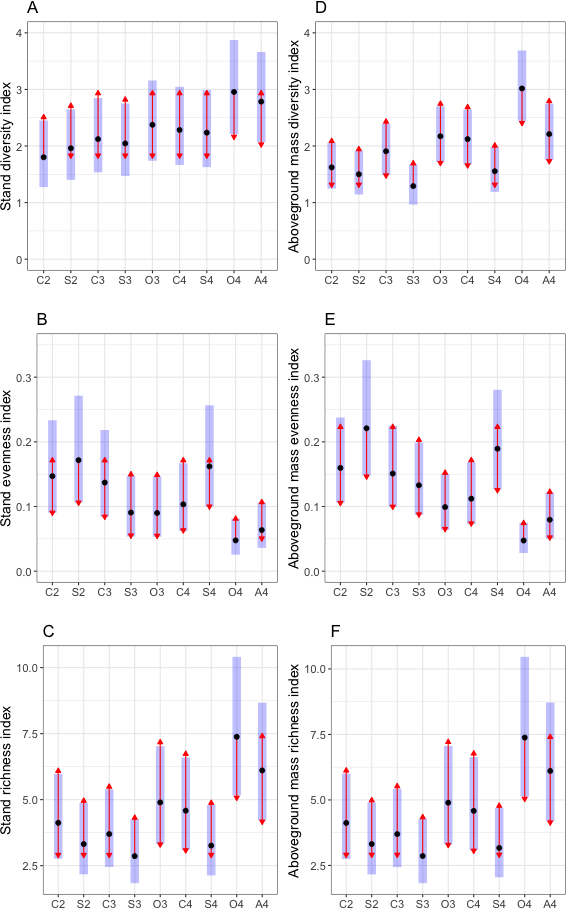
\includegraphics{Community_files/figure-latex/index-arrow-p-1.png}
\caption{\label{fig:index-arrow-p}Weed community stand diversity (A), evenness (B), and richness (C) and community aboveground diversity (D), evenness (E), and richness (F). The abbreviations on the x-axis are crop identities, which are the combinations of the first letter in crop species names and the rotation to which the crops belonged (C2 - corn in the 2-year rotation, C3 - corn in the 3-year rotation, C4 - corn in the 4-year rotation, S2 - soybean in the 2-year rotation, S3 - soybean in the 3-year rotation, S4 - soybean in the 4-year rotation, O3 - oat in the 3-year rotation, O4 - oat in the 4-year rotation, and A4 - alfalfa in the 4-year rotation). The black dots are estimated marginal means. The blue bars are 95\% confidence intervals. The red arrows reflect comparisons among means. Overlapping arrows indicate non-significant differences.}
\end{figure}

\emph{In general, the hypothesis that ``weed communities in the more diverse cropping systems are more diverse'' was supported.}

Averaged over crop phases within each rotation system (Table \ref{tab:dens-indices-ct}A), the weed stand diversity index for the 3-year and 4-year rotation systems was comparable with that in the 2-year rotation (p-values = 0.0535 and 0.1575). For the individual crops (Table \ref{tab:dens-indices-ct}B), the weed stand density diversity index was comparable among rotations (p-values \textgreater{} 0.05). For different crop types (Table \ref{tab:dens-indices-ct}C), the weed stand density diversity index was significantly different between the average for the cool season crops (O3, O4, and A4) and the average for the warm season crops (C2, S2, C3, S3, C4, and S4) (p-value = 0.0145), but similar between the warm season and cool season crops in the same rotations (p-values = 0.4666 and 0.0987). The weed stand density diversity index was similar between oat and alfalfa (p-value = 0.7762).

Averaged over crop phases within the same rotation (Table \ref{tab:biom-indices-ct}A), the weed aboveground mass diversity index was significantly different between the 2-year rotation and the average of the 3-year and 4-year rotations (p-value = 0.0148), and between the 3-year and 4-year rotations (p-value = 0.0209). Averaged over the corn and soybean phases within the same rotation (Table \ref{tab:biom-indices-ct}A), the weed aboveground mass diversity index was similar between rotations (p-values = 0.4217 and 0.2426). For the individual crops (Table \ref{tab:dens-indices-ct}B), the weed aboveground mass diversity index was comparable across rotations, except for oat (p-value = 0.0351). For different crop types (Table \ref{tab:dens-indices-ct}C), the weed aboveground mass diversity index was significantly different between the cool season crops and warm season crops averages (p-values \textless{} 0.0001) and between the cool season and warm season crops within the same rotation (p-values = 0.034 and 0.0037). The weed aboveground mass diversity index was comparable between oat and alfalfa (p-value = 0.2583).

\emph{The hypothesis that ``weed communities in the more diverse cropping systems are more even'' was partially supported (Figure \ref{fig:index-arrow-p}B and E).} However, a lower community evenness index can occur because the presence of rarer species decreases the overall evenness index {[}@stirlingEmpiricalRelationshipsSpecies2001{]}. More details to support this concept are presented later (Figure \ref{fig:all-sp-dens-biom}C and D).

Averaged over crop phases within the same rotation (Table \ref{tab:dens-indices-ct}A), the weed stand density evenness index was significantly different between the 2-year rotation and the average of the 3-year and 4-year rotations (p-value = 0.006), but comparable between the 3-year and 4-year rotations (p-value = 0.2802). Averaged over the corn and soybean phases within the same rotation (Table \ref{tab:dens-indices-ct}A), the weed stand density evenness index was comparable between rotations (p-values = 0.1539 and 0.5031). For the individual crops (Table \ref{tab:dens-indices-ct}B), the weed stand density evenness index was comparable between rotations (p-values \textgreater{} 0.05). For different crop types (Table \ref{tab:dens-indices-ct}C), the weed stand density evenness index was significantly different between the cool season crops average and the warm season crops average (p-value = 0.0002) and between the cool season and warm season crop in the 4-year rotation (p-value = 0.0012), but similar between the warm season and cool season crops in the 3-year rotation (p-values = 0.4418). The weed stand density evenness index was comparable between oat and alfalfa (p-value = 0.8986).

Averaged over crop phases within the same rotation (Table \ref{tab:biom-indices-ct}A), the weed aboveground mass evenness index was significantly different between the 2-year rotation and the average of 3-year and 4-year rotations (p-value = 0.0012), but similar between the 3-year and 4-year rotations (p-value = 0.0802). Averaged over the corn and soybean phases within the same rotation (Table \ref{tab:biom-indices-ct}A), weed aboveground mass evenness index was comparable between rotations (p-values = 0.1081 and 0.8682). For the individual crops (Table \ref{tab:dens-indices-ct}B), the weed aboveground mass evenness index was comparable across rotations (p-values \textgreater{} 0.05), except for oat (p-value = 0.0189). For different crop types (Table \ref{tab:biom-indices-ct}C), the weed aboveground mass evenness index was significantly different between the cool season crops average and the warm season crops average (p-value \textless{} 0.0001) and between the cool season and warm season crops in the 4-year rotation (p-value = 0.0002), but comparable between the warm season and cool season crops in the 3-year rotation (p-values = 0.141). The weed aboveground mass evenness index was comparable between oat and alfalfa (p-value = 0.5911).

\emph{The hypothesis that ``the weed communities in the more diverse cropping systems are more species-rich'' was supported.}

Averaged over crop phases within the same rotation (Table \ref{tab:dens-indices-ct}A), the weed stand density richness index was comparable in the 2-year rotation and in the average of the 3-year and 4-year rotations (p-values = 0.1819), but significantly different between the 3-year and 4-year rotation (p-value = 0.0257). Averaged over the corn and soybean phases within the same rotation (Table \ref{tab:dens-indices-ct}A), weed aboveground mass richness index was comparable between the 2-year rotation and the 3-year and 4-year rotations average (p-value = 0.7996) and between the 3-year and 4-year rotations (p-value = 0.3469). For individual crops (Table \ref{tab:dens-indices-ct}B), the weed stand density richness index was comparable between rotations (p-values \textgreater{} 0.05). For different crop types (Table \ref{tab:dens-indices-ct}C), the weed stand density richness index was significantly different between the cool season crops average and the warm season crops average (p-value = 0.0003) and between the cool season and warm season crops in the 4-year rotation (p-value = 0.0034), but comparable between the warm season and cool season crops in the 3-year rotation (p-values = 0.0725). The weed stand density richness index was comparable between oat and alfalfa (p-value = 0.9499).

Averaged over crop phases within the same rotation (Table \ref{tab:biom-indices-ct}A), the weed aboveground mass richness index was comparable in the 2-year rotation and in the average of the 3-year and 4-year rotations (p-values = 0.1967), but significantly different between the 3-year and 4-year rotations (p-value = 0.0309). Averaged over the corn and soybean phases within the same rotation (Table \ref{tab:biom-indices-ct}A), the weed aboveground mass richness index was comparable between the 2-year rotation and the 3-year and 4-year rotations average (p-value = 0.7694) and between the 3-year and 4-year rotations (p-value = 0.393). For the same crop types, (Table \ref{tab:biom-indices-ct}B), the weed aboveground mass richness index was comparable across rotations (p-values \textgreater{} 0.05). For different crop types (Table \ref{tab:biom-indices-ct}C), the weed aboveground richness index was significantly different between the cool season and warm season crop averages (p-value = 0.0003) and between the cool season and warm season crops in the 4-year rotation (p-value = 0.0766), but comparable between the cool season and warm season crops in the 3-year rotation (p-value = 0.0766). The weed aboveground mass richness index was comparable between oat and alfalfa (p-value = 0.9506).

\begin{table}

\caption{\label{tab:dens-indices-ct}Weed stand density ecological indices contrast significance. The abbreviations on the contrast column are crop identities, which are the combinations of the first letter in crop species names and the rotation to which the crops belonged.}
\centering
\begin{threeparttable}
\begin{tabular}[t]{lrrrlrr}
\toprule
\multicolumn{1}{c}{ } & \multicolumn{2}{c}{Diversity index} & \multicolumn{2}{c}{Evenness index} & \multicolumn{2}{c}{Richness index} \\
\cmidrule(l{3pt}r{3pt}){2-3} \cmidrule(l{3pt}r{3pt}){4-5} \cmidrule(l{3pt}r{3pt}){6-7}
Contrast & ratio & p.value & ratio & p.value & ratio & p.value\\
\midrule
\addlinespace[0.3em]
\multicolumn{7}{l}{\textbf{(A) - Rotation system effects}}\\
\hspace{1em}{}[(C2+S2)/2] vs [(C3+S3+O3+C4+S4+O4+A4)/7] & 0.85 & 0.0535 & 1.60 & 0.0060 & 0.86 & 0.1819\\
\hspace{1em}{}[(C3+S3+O3)/3] vs [(C4+S4+O4+A4)/4] & 0.90 & 0.1575 & 1.18 & 0.2802 & 0.77 & 0.0257\\
\hspace{1em}{}[(C2+S2)/2] vs [(C3+S3+C4+S4)/4] & 0.91 & 0.2749 & 1.28 & 0.1539 & 1.03 & 0.7996\\
\hspace{1em}{}[(C3+S3)/2] vs [(C4+S4)/2] & 0.95 & 0.5824 & 0.88 & 0.5031 & 0.87 & 0.3469\\
\addlinespace[0.3em]
\multicolumn{7}{l}{\textbf{(B) - Rotation system effects within individual crops}}\\
\hspace{1em}C2 vs [(C3+C4)/2] & 0.88 & 0.2836 & 1.20 & 0.4406 & 1.00 & 0.9985\\
\hspace{1em}C3 vs C4 & 0.95 & 0.7231 & 1.28 & 0.3757 & 0.84 & 0.3966\\
\hspace{1em}S2 vs [(S3+S4)/2] & 0.94 & 0.6331 & 1.36 & 0.2065 & 1.06 & 0.7212\\
\hspace{1em}S3 vs S4 & 0.94 & 0.6711 & 0.60 & 0.0746 & 0.91 & 0.6260\\
\hspace{1em}O3 vs O4 & 0.85 & 0.2716 & 1.66 & 0.0757 & 0.70 & 0.0912\\
\addlinespace[0.3em]
\multicolumn{7}{l}{\textbf{(C) - Crop type effects}}\\
\hspace{1em}{}[(O3+O4+A4)/3] vs [(C2+S2+C3+S3+C4+S4)/6] & 1.20 & 0.0145 & 0.55 & 0.0002 & 1.53 & 0.0003\\
\hspace{1em}O3 vs [(C3+S3)/2] & 1.09 & 0.4666 & 0.83 & 0.4418 & 1.38 & 0.0725\\
\hspace{1em}{}[(O4+A4)/2] vs [(C4+S4)/2] & 1.19 & 0.0987 & 0.49 & 0.0012 & 1.58 & 0.0034\\
\hspace{1em}{}[(O3+O4)/2] vs A4 & 0.97 & 0.7762 & 1.03 & 0.8986 & 0.99 & 0.9499\\
\bottomrule
\end{tabular}
\begin{tablenotes}[para]
\item \textit{Note: } 
\item C2 - corn in the 2-year rotation, C3 - corn in the 3-year rotation, C4 - corn in the 4-year rotation, S2 - soybean in the 2-year rotation, S3 - soybean in the 3-year rotation, S4 - soybean in the 4-year rotation, O3 - oat in the 3-year rotation, O4: oat in the 4-year rotation, and A4 - alfalfa in the 4-year rotation
\end{tablenotes}
\end{threeparttable}
\end{table}

\begin{table}

\caption{\label{tab:biom-indices-ct}Weed aboveground mass ecological indices contrast significance. The abbreviations on the contrast column (C2, S2, ..., A4) are crop identities, which are the combinations of the first letter in crop species names and the rotation to which the crops belonged.}
\centering
\begin{threeparttable}
\begin{tabular}[t]{lrrrlrr}
\toprule
\multicolumn{1}{c}{ } & \multicolumn{2}{c}{Diversity index} & \multicolumn{2}{c}{Evenness index} & \multicolumn{2}{c}{Richness index} \\
\cmidrule(l{3pt}r{3pt}){2-3} \cmidrule(l{3pt}r{3pt}){4-5} \cmidrule(l{3pt}r{3pt}){6-7}
Contrast & ratio & p.value & ratio & p.value & ratio & p.value\\
\midrule
\addlinespace[0.3em]
\multicolumn{7}{l}{\textbf{(A) - Rotation system effects}}\\
\hspace{1em}{}[(C2+S2)/2] vs [(C3+S3+O3+C4+S4+O4+A4)/7] & 0.85 & 0.0148 & 1.65 & 0.0012 & 0.86 & 0.1967\\
\hspace{1em}{}[(C3+S3+O3)/3] vs [(C4+S4+O4+A4)/4] & 0.87 & 0.0209 & 1.27 & 0.0802 & 0.78 & 0.0309\\
\hspace{1em}{}[(C2+S2)/2] vs [(C3+S3+C4+S4)/4] & 0.95 & 0.4217 & 1.28 & 0.1081 & 1.04 & 0.7694\\
\hspace{1em}{}[(C3+S3)/2] vs [(C4+S4)/2] & 0.91 & 0.2426 & 0.97 & 0.8682 & 0.88 & 0.3930\\
\addlinespace[0.3em]
\multicolumn{7}{l}{\textbf{(B) - Rotation system effects within individual crops}}\\
\hspace{1em}C2 vs [(C3+C4)/2] & 0.87 & 0.1425 & 1.20 & 0.3825 & 1.00 & 0.9985\\
\hspace{1em}C3 vs C4 & 0.93 & 0.5084 & 1.31 & 0.2780 & 0.84 & 0.4035\\
\hspace{1em}S2 vs [(S3+S4)/2] & 1.03 & 0.7219 & 1.36 & 0.1543 & 1.08 & 0.6801\\
\hspace{1em}S3 vs S4 & 0.90 & 0.3166 & 0.72 & 0.1905 & 0.93 & 0.7075\\
\hspace{1em}O3 vs O4 & 0.79 & 0.0351 & 1.83 & 0.0189 & 0.70 & 0.0957\\
\addlinespace[0.3em]
\multicolumn{7}{l}{\textbf{(C) - Crop type effects}}\\
\hspace{1em}{}[(O3+O4+A4)/3] vs [(C2+S2+C3+S3+C4+S4)/6] & 1.30 & <.0001 & 0.51 & <.0001 & 1.54 & 0.0003\\
\hspace{1em}O3 vs [(C3+S3)/2] & 1.23 & 0.0340 & 0.73 & 0.1410 & 1.38 & 0.0766\\
\hspace{1em}{}[(O4+A4)/2] vs [(C4+S4)/2] & 1.27 & 0.0037 & 0.48 & 0.0002 & 1.60 & 0.0032\\
\hspace{1em}{}[(O3+O4)/2] vs A4 & 1.11 & 0.2583 & 0.89 & 0.5911 & 0.99 & 0.9506\\
\bottomrule
\end{tabular}
\begin{tablenotes}[para]
\item \textit{Note: } 
\item C2 - corn in the 2-year rotation, C3 - corn in the 3-year rotation, C4 - corn in the 4-year rotation, S2 - soybean in the 2-year rotation, S3 - soybean in the 3-year rotation, S4 - soybean in the 4-year rotation, O3 - oat in the 3-year rotation, O4 - oat in the 4-year rotation, and A4 - alfalfa in the 4-year rotation
\end{tablenotes}
\end{threeparttable}
\end{table}

\hypertarget{general-description-of-the-weed-flora}{%
\paragraph*{General description of the weed flora}\label{general-description-of-the-weed-flora}}
\addcontentsline{toc}{paragraph}{General description of the weed flora}

Overall, 34 weed species were identified during the four years of data collection (Table \ref{tab:list-sp}). Combined over four years of data, seven weed species, SETFA (\emph{Setaria faberi}), AMATA (\emph{Amaranthus tuberculatus}), CHEAL (\emph{Chenopodium album}), DIGSA (\emph{Digitaria sanguinalis}), ECHCG (\emph{Echinochloa crus-galli}), SETLU (\emph{Setaria glauca}), and TAROF (\emph{Taraxacum officinale}) made up 94.4\% of the total weed density and 94.0\% of the total weed biomass (Figure \ref{fig:all-sp-dens-biom}C and D).

\begin{table}

\caption{\label{tab:list-sp}List of weed species (in alphabetical order) found from 2017 to 2020 field seasons.}
\centering
\begin{tabular}[t]{l|l|l}
\hline
Bayer code & Scientific name & Life cycle\\
\hline
\multicolumn{3}{l}{\textbf{(A) - Dicotyledon species}}\\
\hline
\hspace{1em}ABUTH & $Abutilon~theophrasti$$~$ Medicus & annual\\
 
\hspace{1em}AMARE & $Amaranthus~retrofelxus$$~$ L. & summer annual\\
 
\hspace{1em}AMATA & $Amaranthus~tuberculatus$$~$ (Moq.) Sauer~var.~$rudis$ & summer annual\\
 
\hspace{1em}AMBEL & $Ambrosia~artemissifolia$$~$ L. & erect, branching, summer annual\\
 
\hspace{1em}ARFMI & $Arctium~minus$$~$ (Hill) Bernh. & biennial\\
 
\hspace{1em}CHEAL & $Chenopodium~album$$~$ L. & erect summer annual\\
 
\hspace{1em}CIRAR & $Cirsium~arvense$$~$ (L.) Scop. & rhizomatous perennial\\
 
\hspace{1em}CIRVU & $Cirsium~vulgare$$~$ (Savi) Tenore & biennial\\
 
\hspace{1em}EPHHT & $Euphorbia~humistrata$$~$ Engelm.$~$ex$~$Gray & mat-forming summer annual\\
 
\hspace{1em}EPHMA & $Euphorbia~maculata$$~$ L. & mat-forming summer annual\\
 
\hspace{1em}EUPHY & $Eupatorium~hyssopifolium$$~$ L. & summer annual\\
 
\hspace{1em}MORAL & $Morus~alba$$~$ L. & perennial shrub\\
 
\hspace{1em}PHYSU & $Physalis~subglabrata$$~$ Mackenz. and Bush & rhizomatous perennial\\
 
\hspace{1em}PLAMA & $Plantago~major$$~$ L. & rosette-forming perennial\\
 
\hspace{1em}POLPY & $Polygonum~pensylvanicum$$~$ L. & ascending much-branched summer annual\\
 
\hspace{1em}POPDE & $Polygonum~perfoliatum$$~$ L. & spiny summer annual vine\\
 
\hspace{1em}POROL & $Portulaca~oleracea$$~$ L. & prostrate mat-forming summer annual\\
 
\hspace{1em}SOLPT & $Solanum~ptycanthum$$~$ Dun. & erect branching summer annual\\
 
\hspace{1em}SONAR & $Sonchus~arvensis$$~$ L. & rhizomatous perennial\\
 
\hspace{1em}TAROF & $Taraxacum~officinale$$~$Weberin$~$Wiggers & tap-rooted perennial\\
 
\multicolumn{3}{l}{\textbf{(B) - Monocotyledon species}}\\
\hline
\hspace{1em}\hspace{1em}AGRRE & $Elytrigia~repens$$~$ (L.) Nevski & rhizomatous perennial\\
 
\hspace{1em}BROTE & $Bromus~tectorum$$~$ L. & summer or winter annual\\
 
\hspace{1em}CCHPA & $Cenchrus~longispinus$$~$ (Hack.) Fern. & summer annual\\
 
\hspace{1em}CONAR & $Convolvulus~arvensis$$~$ L. & rhizomatous perennial\\
 
\hspace{1em}CYPES & $Cyperus~esculentus$$~$ L. & rhizomatous perennial\\
 
\hspace{1em}DACGL & $Dactylis~glomerata$$~$ L. & chump-forming perennial\\
 
\hspace{1em}DIGSA & $Digitaria~sanguinalis$$~$~(L.)~Scop. & summer annual\\
 
\hspace{1em}ECHCG & $Echinochloa~crus-galli$$~$ (L.) Beauv. & summer annual\\
 
\hspace{1em}ERBVI & $Eriochloa~villosa$$~$ (Thunb.) Kunth & erect summer annual\\
 
\hspace{1em}FESSP & $Festuca$$~$ spp. & clump-forming perennial\\
 
\hspace{1em}PANCA & $Panicum~capillare$$~$ L. & summer annual\\
 
\hspace{1em}PANDI & $Panicum~dichotomiflorum$$~$Michx. & summer annual\\
 
\hspace{1em}SETFA & $Setaria~faberi$$~$ Herrm. & clump-forming, erect summer annual\\
 
\hspace{1em}SETLU & $Setaria~glauca$$~$ (L.) Beauv. & clump-forming, erect summer annual\\
\hline
\end{tabular}
\end{table}

\hypertarget{how-did-rotation-crop-species-and-corn-weed-management-affect-weed-community-density-and-growth}{%
\paragraph*{How did rotation, crop species, and corn weed management affect weed community density and growth?}\label{how-did-rotation-crop-species-and-corn-weed-management-affect-weed-community-density-and-growth}}
\addcontentsline{toc}{paragraph}{How did rotation, crop species, and corn weed management affect weed community density and growth?}

Crop identity had a significant effect on weed community stand density (p-value \textless{} 0.0001) and weed aboveground mass (p-value = 0.0057), but corn weed management and its interaction with crop identity did not have a significant effect on weed community stand density or biomass (p-values \textgreater{} 0.05) (Table \ref{tab:dens-indices-ct} and \ref{tab:biom-indices-ct}). Weed total stand density and aboveground mass in each crop identity category, averaged over blocks, years, and corn weed management regimes, are presented in Figure \ref{fig:all-sp-dens-biom}A and B. Contribution by the dominant species are presented in Figure \ref{fig:all-sp-dens-biom}C and D. Contrasts for the effects of rotation systems, rotation system within individual crops, and crop types on community stand density and aboveground mass are shown in Table \ref{tab:dens-biom-jt-ct}C.

Weed community density and aboveground mass of the 3-year and 4-year systems averages were comparable to those of the 2-year system (p-values = 0.058 and 0.9451, Table \ref{tab:dens-biom-jt-ct}B1). The weed density in the 4-year rotation was 2.5 fold greater than in the 3-year rotation (p-value = 0.0368), but the aboveground mass was comparable between the 3-year and 4-year rotations.

For the individual crops (Table \ref{tab:dens-biom-jt-ct}B2), increased rotation diversity tended to decrease weed abundance in corn and soybean and increase weed abundance in oat, but these trends were not significant (p-values = 0.6354 and 0.4041 for corn, 0.1834 and 0.0739 for soybean, and 0.3955 and 0.335 for oat). The patchiness of weeds, which was reflected in the high standard error values, might have caused the lack of significance for these inconclusive trends.

For different crop types (Table \ref{tab:dens-biom-jt-ct}B3), weed community density and aboveground mass were comparable between the warm season crops (corn and soybean, p-values = 0.2032, 0.3426, 0.065, and 0.1274) and between the cool season crops (oat and alfalfa, p-values = 0.774 and 0.687). Overall, the average weed community density in the cool season crops was 26-fold greater than that in the warm season crops (p-value \textless{} 0.0001), and the average weed aboveground mass in cool season crops was 16-fold greater than that in warm season crops (p-value = 0.0001). In the 3-year rotation, the weed stand community stand in oat (O3) was 11.5-fold greater than the average in corn and soybean (C3 and S3) (p-value = 0.0012), but the weed community total aboveground mass was comparable between O3 and the average of the C3 and S3 phases (p-value = 0.1502). In the 4-year rotation, the weed community stand density in the average of oat and alfalfa (O4 and A4) was 36-fold greater than the average of the corn (C4) and soybean (S4) phases (p-value \textless{} 0.0001), and the average weed biomass for the O4 and A4 phases was 29-fold greater than for the C4 and S4 phases (p-value \textless{} 0.0001).

\begin{table}

\caption{\label{tab:dens-biom-jt-ct}Community density and aboveground mass ANOVA and contrasts. The abbreviations in the contrast column are crop identities, which are the combinations of the first letter in crop species names and the rotation to which the crops belonged.}
\centering
\begin{threeparttable}
\begin{tabular}[t]{lrrrrrr}
\toprule
\multicolumn{3}{c}{ } & \multicolumn{2}{c}{Stand density} & \multicolumn{2}{c}{Aboveground mass} \\
\cmidrule(l{3pt}r{3pt}){4-5} \cmidrule(l{3pt}r{3pt}){6-7}
Source of variation & df1 & df2 & F.value & p.value & F.value & p.value\\
\midrule
\addlinespace[0.3em]
\multicolumn{7}{l}{\textbf{(A) - ANOVA}}\\
\hspace{1em}Crop ID & 8 & 24 & 12.22 & <.0001 & 3.74 & 0.0057\\
 
\hspace{1em}Corn weed management & 1 & 3 & 2.13 & 0.2402 & 0.02 & 0.8900\\
 
\hspace{1em}Crop ID x Corn weed management & 8 & 24 & 1.66 & 0.1613 & 0.99 & 0.4660\\
 
\addlinespace[0.3em]
\multicolumn{7}{l}{\textbf{Contrasts                 ratio  p.value  ratio   p.value}}\\
\addlinespace[0.3em]
\multicolumn{7}{l}{\textbf{(B1) - Rotation system effects}}\\
\hspace{1em}\hspace{1em}{}[(C2+S2)/2] vs [(C3+S3+O3+C4+S4+O4+A4)/7] &  &  & 0.42 & 0.0580 & 0.96 & 0.9451\\
 
\hspace{1em}\hspace{1em}{}[(C3+S3+O3)/3] vs [(C4+S4+O4+A4)/4] &  &  & 0.40 & 0.0368 & 0.42 & 0.1712\\
 
\addlinespace[0.3em]
\multicolumn{7}{l}{\textbf{(B2) - Rotation system effects within individual crops}}\\
\hspace{1em}\hspace{1em}C2 vs [(C3+C4)/2] &  &  & 1.38 & 0.6354 & 2.30 & 0.4041\\
 
\hspace{1em}\hspace{1em}C3 vs C4 &  &  & 0.59 & 0.4969 & 0.73 & 0.7853\\
 
\hspace{1em}\hspace{1em}S2 vs [(S3+S4)/2] &  &  & 2.49 & 0.1834 & 6.25 & 0.0739\\
 
\hspace{1em}\hspace{1em}S3 vs S4 &  &  & 1.19 & 0.8248 & 1.04 & 0.9731\\
 
\hspace{1em}\hspace{1em}O3 vs O4 &  &  & 0.51 & 0.3955 & 0.33 & 0.3350\\
 
\addlinespace[0.3em]
\multicolumn{7}{l}{\textbf{(B3) - Crop type effects}}\\
\hspace{1em}\hspace{1em}{}[(C2+S2)/2] vs [(C3+S3+C4+S4)/4] &  &  & 1.85 & 0.2032 & 3.79 & 0.0665\\
 
\hspace{1em}\hspace{1em}{}[(C3+S3)/2] vs [(C4+S4)/2] &  &  & 1.69 & 0.3426 & 3.54 & 0.1274\\
 
\hspace{1em}\hspace{1em}{}[(O3+O4+A4)/3] vs [(C2+S2+C3+S3+C4+S4)/6] &  &  & 26.10 & <.0001 & 16.00 & 0.0001\\
 
\hspace{1em}\hspace{1em}O3 vs [(C3+S3)/2] &  &  & 11.50 & 0.0012 & 4.29 & 0.1502\\
 
\hspace{1em}\hspace{1em}{}[(O4+A4)/2] vs [(C4+S4)/2] &  &  & 35.90 & <.0001 & 28.70 & 0.0003\\
 
\hspace{1em}\hspace{1em}{}[(O3+O4)/2] vs A4 &  &  & 0.80 & 0.7440 & 1.49 & 0.6870\\
\bottomrule
\end{tabular}
\begin{tablenotes}[para]
\item \textit{Note: } 
\item C2 - corn in the 2-year rotation, C3 - corn in the 3-year rotation, C4 - corn in the 4-year rotation, S2 - soybean in the 2-year rotation, S3 - soybean in the 3-year rotation, S4 - soybean in the 4-year rotation, O3 - oat in the 3-year rotation, and O4 - oat in the 4-year rotation.
\end{tablenotes}
\end{threeparttable}
\end{table}

\begin{figure}
\centering
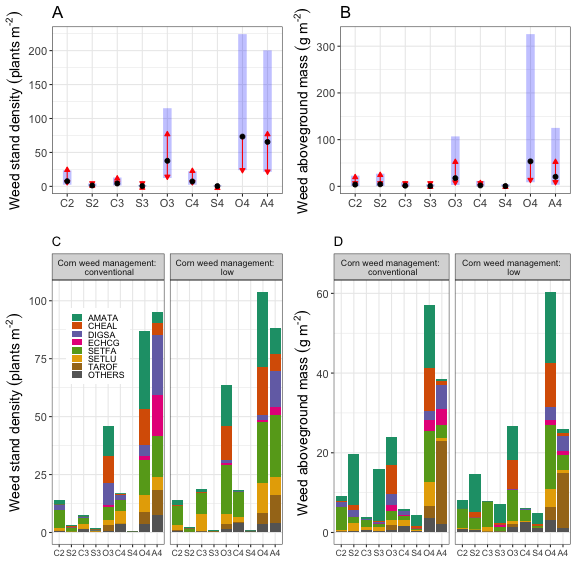
\includegraphics{Community_files/figure-latex/all-sp-dens-biom-1.png}
\caption{\label{fig:all-sp-dens-biom}In panels A and B: weed community stand density and aboveground mass were averaged over four blocks, four years, and two corn weed management regimes; the black dots are estimated marginal means; the blue bars are 95\% confidence intervals; the red arrows reflect the comparisons among means; overlapping arrows indicate non-significant differences. In panels C and D: the contribution of the seven most abundant weed species and the rarer species (species ordered eighth and above grouped in OTHERS) in each crop identity, averaged over four blocks and four years, are ordered alphabetically. The abbreviations on the x-axis are crop identities, which are the combinations of the first letter in crop species names and the rotation to which the crops belonged (C2 - corn in the 2-year rotation, C3 - corn in the 3-year rotation, C4 - corn in the 4-year rotation, S2 - soybean in the 2-year rotation, S3 - soybean in the 3-year rotation, S4 - soybean in the 4-year rotation, O3 - oat in the 3-year rotation, O4 - oat in the 4-year rotation, and A4 - alfalfa in the 4-year rotation.) The less abundant weed species which made up 6\% of the whole community are grouped in OTHERS. The means displayed on panels A and B were estimated marginal means, calculated based on the analysis model (with \texttt{emmip} function) but the means displayed on panels C and D were arithmetic means, calculated from the data so they are slightly different.}
\end{figure}

\end{document}
